\documentclass[10pt]{article}
\usepackage{icmlko}

\icmlmeta{IP 파운데이션 월드모델}{301}{빈 칸인 줄 알았더니 기둥이었다}{노트 300이 잡음이라 부른 마흔일곱 자리를 껐더니 판이 갈릴 만큼 나빠졌다 --- 파운데이션 주장의 첫 직접 증거}

\begin{document}

\twocolumn[
\icmlheader

\begin{abstract}
노트 300이 채택 검사 ③ 을 판 전체에 돌려 잴 수 있는 100자리 중 \textbf{47을
``안 오른다''}로 판정하고 표에 \textbf{잡음}이라고 적었다. 껐다. 사전 등록해
놓고(\texttt{preregister\_maskdead.json}) 예상은 \textbf{``거의 안 움직인다,
판 $|\Delta|{<}0.005$''}였다. \textbf{반대였다} --- 판 0.4851 $\to$
\textbf{0.4730}, $\Delta{=}{-}0.0121$, 짝SE 0.0047, $t{=}{-}2.58$, 문턱
0.0094. \textbf{갈린다. 나빠졌다.} 그리고 무너지는 자리가 뚜렷하다:
\textbf{도서 $-$0.1306}($t{=}{-}2.88$, 9축 끔) · \textbf{펀딩 $-$0.1221}
($t{=}{-}2.33$, 9축) --- 노트 300이 ``새로운 축이 0개''라고 지목한 바로 그
두 도메인이다. \textbf{자기 라벨과 주변 관계가 없는 축이 유보에서
0.12$\sim$0.13 $\rho$ 를 지고 있었다.} 갈랐다(노트 133). \textbf{① 값이
일한다} --- 관측 표시자를 남기고 값만 중립 0.5 로 만들어도 똑같이 무너진다
(도서 0.2444 · 펀딩 0.1127). \textbf{② 국지적이다} --- \emph{도서만} 끄면
도서만 $-$0.1381($t{=}{-}2.94$)이고 펀딩 · 애니는 안 움직인다. 전역 적합이
바뀐 탓이 아니라 \textbf{그 도메인의 행이 그 값을 쓴다.} 남는 경로는 하나다
--- 웹툰 · 애니에서 배운 분할이 도서 · 펀딩 행에 \textbf{건너가서} 쓰인다.
\textbf{이 실험실이 파운데이션 주장에 대해 처음 얻은 직접 증거다.} 그리고
\textbf{한계 검정은 축의 값어치를 못 잰다} --- 노트 300의 표에서 ``잡음''을
지운다.
\end{abstract}
]

\section{잡음이라 적어 놓고 껐다}

노트 300이 도메인 $\times$ 축 184자리를 판정하고 이렇게 적었다.

\begin{center}\footnotesize
\begin{tabular}{ll}
\hline
자리 & \textbf{노트 300이 적은 것} \\
\hline
새롭다 36 & 정보를 나른다 \\
이미 있다 17 & 같은 말을 두 번 \\
안 오른다 47 & \textbf{잡음} \\
\hline
\end{tabular}
\end{center}

껐다. 그 (도메인, 축)의 마스크를 0 으로 만들면 \texttt{forms.\_design} 이
값 0.5 · 표시자 0 으로 읽는다 --- ``이 도메인은 그 축을 모른다''다. 판정
근거가 \textbf{학습 구간}이므로 유보를 안 보고 고를 수 있다(노트 239 · 242).

\paragraph{예상을 먼저 적었다} ``\textbf{거의 안 움직인다.} 판
$|\Delta|{<}0.005$. 나무는 관계없는 열을 쓸 이유가 없고, 노트 292의 사례는
열이 라벨과 \emph{인공적으로 상관된} 경우였지 무관한 경우가 아니었다.''

\section{나빠졌다}

\begin{figure*}[t]
\centering
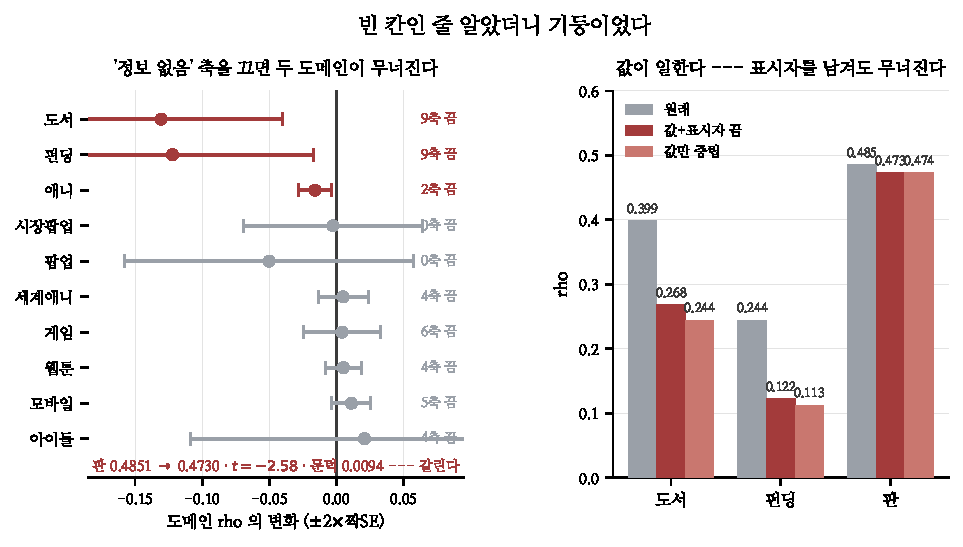
\includegraphics[width=\textwidth]{figs/load.pdf}
\caption{왼쪽 --- ``안 오른다'' 자리를 껐을 때 도메인 $\rho$ 의 변화
($\pm$2$\times$짝SE, 부트스트랩 400). 오른쪽 --- 값과 표시자를 갈라 끈 것.}
\end{figure*}

\begin{center}\small
\begin{tabular}{lr}
\hline
판 (원래) & 0.4851 \\
판 (47자리 끔) & \textbf{0.4730} \\
\hline
$\Delta$ & \textbf{$-$0.0121} \\
짝SE & 0.0047 \\
$t$ & \textbf{$-$2.58} \\
검출 문턱 & 0.0094 \\
\hline
\end{tabular}
\end{center}

\textbf{문턱을 넘는다. 갈린다.} 오늘 열 번 가까이 ``문턱 아래''로 끝냈는데
이번엔 넘었고 \textbf{방향이 반대다.}

\begin{center}\footnotesize
\begin{tabular}{lrrrr}
\hline
도메인 & 원래 & 막음 & $\Delta$ & $t$ \\
\hline
\textbf{도서} & 0.3988 & 0.2682 & \textbf{$-$0.1306} & \textbf{$-$2.88} \\
\textbf{펀딩} & 0.2444 & 0.1223 & \textbf{$-$0.1221} & $-$2.33 \\
애니 & 0.5012 & 0.4853 & $-$0.0159 & $-$2.61 \\
팝업 & 0.3750 & 0.3250 & $-$0.0500 & $-$0.93 \\
모바일 & 0.5435 & 0.5547 & $+$0.0112 & $+$1.54 \\
아이돌 & 0.0751 & 0.0961 & $+$0.0210 & $+$0.32 \\
웹툰 & 0.4619 & 0.4671 & $+$0.0053 & $+$0.79 \\
세계애니 & 0.5336 & 0.5387 & $+$0.0051 & $+$0.55 \\
게임 & 0.6214 & 0.6258 & $+$0.0044 & $+$0.31 \\
\hline
\end{tabular}
\end{center}

도메인 문턱($|t|{>}2.77$)을 넘는 것은 \textbf{도서} 하나지만, 크기로 보면
\textbf{도서와 펀딩이 각각 $\rho$ 0.12$\sim$0.13 을 잃는다.} 그리고 그 둘이
노트 300이 ``새로운 축이 0개''로 지목한 바로 그 도메인이다. \textbf{새로운
게 없다던 자리가 제일 크게 무너졌다.}

가드 열아홉 \textbf{통과}(마스크를 0 으로 만드는 것이 출처 무늬를 만들지
않았다).

\section{갈랐다 --- 값이고, 국지적이다}

첫 수치를 그대로 채택하지 않는다(노트 133). 두 갈래를 쟀다.

\paragraph{① 값이냐 표시자냐} 관측 표시자를 \textbf{남기고} 값만 중립
0.5 로 만들어 봤다.

\begin{center}\footnotesize
\begin{tabular}{lrrr}
\hline
& 원래 & 값$+$표시자 끔 & \textbf{값만 중립} \\
\hline
도서 & 0.3988 & 0.2682 & \textbf{0.2444} \\
펀딩 & 0.2444 & 0.1223 & \textbf{0.1127} \\
판 & 0.4851 & 0.4730 & 0.4736 \\
\hline
\end{tabular}
\end{center}

\textbf{똑같이 무너진다} --- 오히려 조금 더. \textbf{값이 일한다.} ``이
도메인이 달력 자료를 갖고 있다''는 사실 자체가 아니라 \emph{그 달력 값}이
쓰이고 있다.\footnote{표시자만 끄고 값을 남기는 팔은 이 설계에서 만들 수
없다 --- \texttt{\_design} 이 마스크 0 이면 값을 0.5 로 덮는다. 그래서
그 팔의 수는 ``둘 다 끔''과 정확히 같게 나온다.}

\paragraph{② 전역이냐 국지냐} 마스크를 \textbf{한 도메인에만} 걸어 봤다.

\begin{center}\footnotesize
\begin{tabular}{lrrrr}
\hline
끈 도메인 & 도서 & 펀딩 & 애니 & 판 \\
\hline
없음 & 0.3988 & 0.2444 & 0.5012 & 0.4851 \\
\textbf{도서만} & \textbf{0.2606} & 0.2602 & 0.4980 & 0.4785 \\
\textbf{펀딩만} & 0.3956 & \textbf{0.1375} & 0.5003 & 0.4774 \\
애니만 & 0.3959 & 0.2424 & 0.4975 & 0.4842 \\
전부 & 0.2682 & 0.1223 & 0.4853 & 0.4730 \\
\hline
\end{tabular}
\end{center}

\textbf{도서만 끄면 도서만 무너진다}($-$0.1381 · $t{=}{-}2.94$). 펀딩 · 애니는
안 움직인다. 펀딩도 같다($-$0.1069 · $t{=}{-}1.95$). \textbf{전역 적합이 바뀐
탓이 아니다.}

다만 아주 없지는 않다 --- 애니는 \emph{자기만} 끌 때 $-$0.0037($t{=}{-}1.06$)
인데 \emph{전부} 끌 때 $-$0.0159 다. 차 0.012 가 \textbf{남의 도메인을 끈
탓}이다. 공유 적합이 실재한다는 또 다른 흔적이다.

\section{그래서 파운데이션 주장의 첫 직접 증거다}

남는 설명은 하나다.

\begin{center}\small
\begin{tabular}{l}
\hline
도서의 \texttt{cal\_*} 는 \textbf{도서 라벨과 관계가 없다}($p{>}0.05$) \\
그런데 도서의 유보 $\rho$ 를 \textbf{0.14} 지고 있다 \\
그리고 그것은 \textbf{도서 행에서만} 일어난다 \\
\hline
$\Rightarrow$ 웹툰 · 애니에서 배운 분할이 \textbf{건너와서} \\
\quad 도서 행의 그 값에 적용된다 \\
\hline
\end{tabular}
\end{center}

이 실험실은 ``IP $\cdot$ 기획 $\to$ 소비자 반응''을 도메인 가로질러 배우겠다는
목표로 돌아 왔고, 노트 291 · 293 · 294가 크로스 도메인 \emph{자료}(같은 IP ·
같은 회사)를 찾다가 전부 문턱 아래로 끝났다. \textbf{그런데 전이는 자료가
아니라 축을 통해 이미 일어나고 있었다} --- 그리고 그 크기가 0.12$\sim$0.13
이다. 오늘 잰 어떤 것보다 크다.

\section{노트 300의 표를 고친다}

\begin{center}\footnotesize
\begin{tabular}{lll}
\hline
자리 & 노트 300 & \textbf{고침} \\
\hline
새롭다 36 & 정보를 나른다 & 그대로 \\
이미 있다 17 & 같은 말 두 번 & 그대로 \\
안 오른다 47 & \textbf{잡음} & \textbf{빌려 쓰는 자리} \\
\hline
\end{tabular}
\end{center}

\textbf{한계 검정은 축의 값어치를 못 잰다.} 스피어만 · 크루스칼은 ``이 축이
\emph{이 도메인에서} 혼자 라벨을 가르나''를 묻는데, 파운데이션 모형에서 축의
일은 \textbf{다른 도메인에서 배운 함수의 입력이 되는 것}이다. 그 일은 자기
도메인 안의 주변 관계로는 안 보인다.

\paragraph{그러면 검사 ③ 은 무엇인가} 여전히 유효하다 --- 노트 299의
\texttt{mkt\_cat} 은 ``\textbf{이미 있다}''(① 통과 ③ 탈락)였고 그건 다른
판정이다. 이번에 무너진 것은 ``\textbf{안 오른다}''(① 탈락)다.
\textbf{① 을 이유로 축을 빼면 안 된다}가 이 노트의 결론이고, ③ 은 그대로 둔다.

\paragraph{남은 것}
\begin{center}\small
\begin{tabular}{ll}
\hline
갈래 & 왜 \\
\hline
빌림을 크기로 재라 & 도메인마다 얼마를 빌리나 \\
``이미 있다'' 17 도 껐을 때 & ③ 도 같은 함정인가 \\
작은 다섯에 축을 더 & 빌릴 자리가 더 있다는 뜻 \\
위약 팔 & 신호가 내용이냐 모양이냐 \\
\hline
\end{tabular}
\end{center}

\paragraph{규약} \textbf{축을 뺄 때는 넣을 때보다 더 세게 물어라.} 노트 300은
축 \emph{자리}를 판정만 했는데 표의 낱말 하나(``잡음'')가 곧바로 다음 수를
정했고, 그 다음 수가 판을 0.0121 떨어뜨렸다. \textbf{판정과 처방은 다른
측정이다.} 그리고 \textbf{한 도메인 안에서 안 보이는 것이 없는 것은 아니다}
--- 이 판의 설계 전체가 ``남에게서 배워 여기에 쓴다''인데, 그 이득을
\emph{여기 안에서만} 재고 있었다.

\end{document}
